\documentclass[../monografia.tex]{subfiles}
\graphicspath{ {images/}{../images/} } 

\begin{document}
% Detalhar neste item os procedimentos realizados para os testes de funcionamento dos sub-sistemas, da inter-relação dos subsistemas e do sistema completo.

\section{Resultados dos Testes}
\section{Verificação dos requisitos}

\begin{figure}[h!]
	\centering
	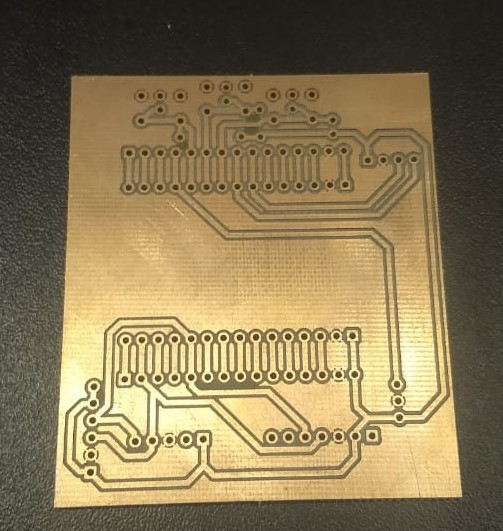
\includegraphics[width=10cm]{pcb-fresada}
	\caption{PCB fresada}
	\label{fig:img5}
	\end{figure}
	
%? Montagem final da placa

\begin{figure}[h]
	\centering
	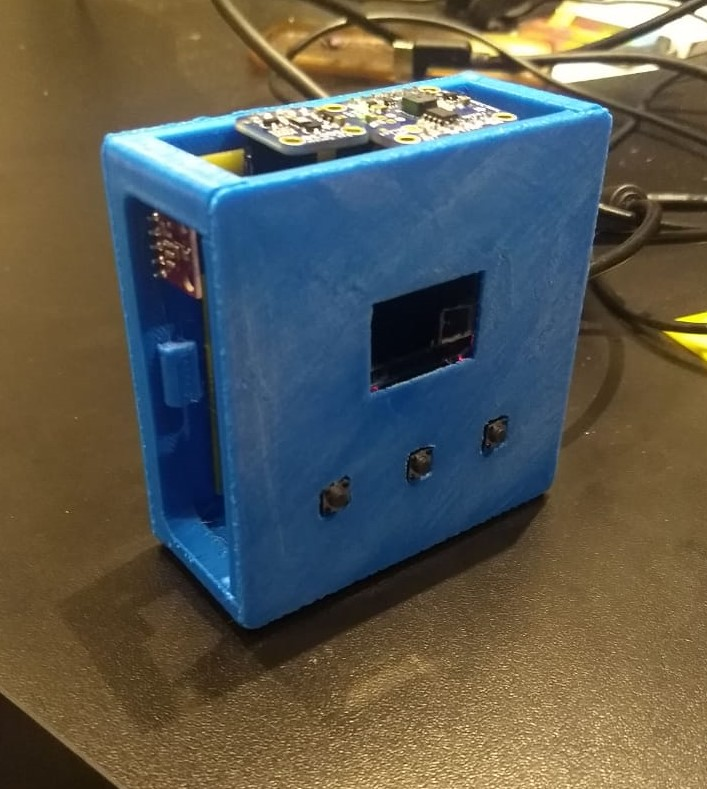
\includegraphics[width=0.8\textwidth]{montagem-final.jpg}
	\caption{Montagem final do protótipo}
	\label{fig:prototipo}
\end{figure}

\section{Futuro?}
\subsection{Harware}
\subsubsection{Alimentação}
(copiado)
Bateria de Lítio-Polímero, de uma célula (1S), por ter a maior densidade energética dentre as baterias recarregáveis, permitindo que o dispositivo seja portátil e não dependente da rede elétrica. A capacidade da bateria será definida com base nos testes de consumo do equipamento nas etapas finais de desenvolvimento do protótipo. 

A bateria LiPo tem tensões de operação entre 3.5 e 4.2 Volts. Para alimentar o circuito foi optado por elevar a tensão para 5V, através de um regulador chaveado boost, ainda não definido. 

Para fazer a recarga da bateria de forma eficiente e segura, foi pensado em um circuito carregador utilizando o CI TP4056 \cite{tp4056}, alimentado por 5V através de um conector USB-micro. Com esse CI é possível também que o circuito opere enquanto a bateria está sendo recarregada. 

\end{document}